\documentclass[twocolumn,10pt]{article}
\title{Composing and Decomposing Shapes 1}
\setlength{\columnsep}{20pt} 
\usepackage{amsmath,hyperref,cancel,graphicx}
 \def\shrinkfactor{0.55}
 \usepackage[margin=1.5cm]{geometry}
\usepackage[usenames,dvipsnames]{color}
 
 \newcommand{\blue}[1]{{\color{Blue}#1}} 
 \newcommand{\purple}[1]{{\color{Purple}#1}} 
 \newcommand{\red}[1]{{\color{Red}#1}} 
 \newcommand{\green}[1]{{\color{Green}#1}} 
 \newcommand{\gray}[1]{{\color{Gray}#1}} 
  \newcommand{\pink}[1]{{\color{Magenta}#1}}   


\begin{document}
\maketitle



\section{\href{https://www.khanacademy.org/devadmin/content/items/x00ceb76b3c63886f}{x00ceb76b3c63886f}}

\noindent
William is cutting the grass.  The picture below, which is measured in acres, represents the area that she has cut.    

**How many square acres of grass has William cut?**  


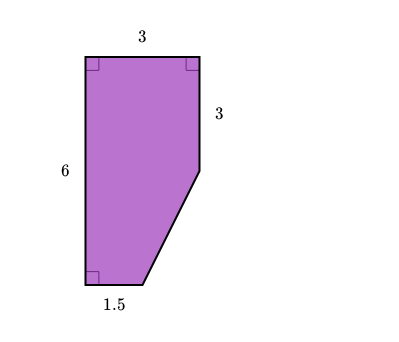
\includegraphics[scale=\shrinkfactor]{figures/151cda9731a44833829ae8798b9679400b8e39bd.png}

\paragraph{Ans}  [[? input-number 1]] $\text{acres}^2$  7

\paragraph{Hint 1}This shape is made up of a square at the top, a rectangle on the left side, and a triangle on the right side.    


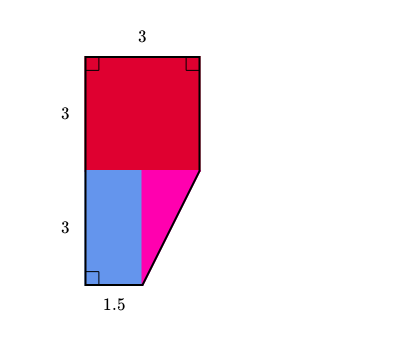
\includegraphics[scale=\shrinkfactor]{figures/302942f7714d41d6f87fcf9150ccaf8be7c6b3f0.png}   
 
We know the square at the top of the shape has a side length of $3$ acres.

$\red{\text{Area}}=\red3\cdot\red3=9\text{ acres}^2$


We know the rectangle on the left side has a length of $3$ acres and a width of $1.5$ acres.   

$\blue{\text{Area}}=\blue3\cdot\blue1\blue.\blue5=4.5\text{ acres}^2$  

The triangle on the right side is one-half of another rectangle:  


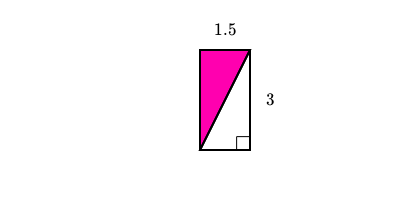
\includegraphics[scale=\shrinkfactor]{figures/75c917243eabb4347d75f1ef3e5c2b8da0da49c8.png}  

$\pink{\text{Area}}=\dfrac{1}{2}\cdot\pink3\cdot\pink1\pink.\pink5=\dfrac{1}{2}\cdot4.5\text{ acres}^2=2.25\text{ acres}^2$

\paragraph{Hint 2}To find the total area of the shape, we can combine the three areas we found:  

$\red9+\blue4\blue.\blue5+\pink2\pink.\pink2\pink5=\purple7$  

The area of this figure is $\purple1\purple5\purple.\purple7\purple5$ square acres.  

\paragraph{Hint 3}William has cut $15.75$ $\text{ acres}^2$ in total.



\medskip
\noindent
\textbf{Tags:} {\footnotesize CC.6.G.A.1, i.	Composing and Decomposing Shapes 1.1, SB.6.1.H.1.CR}\\
\textbf{Version:} 1e4ed40a.. 2013-10-11
\smallskip\hrule





\section{\href{https://www.khanacademy.org/devadmin/content/items/x1360b3084d511d3f}{x1360b3084d511d3f}}

\noindent
Matthew drew a picture of his house on construction paper.  He needs $6$ figures exactly the same size and shape as the house, which is measured in inches. **Using the model below, how many square inches of paper will his $6$ figures measure in total?**    


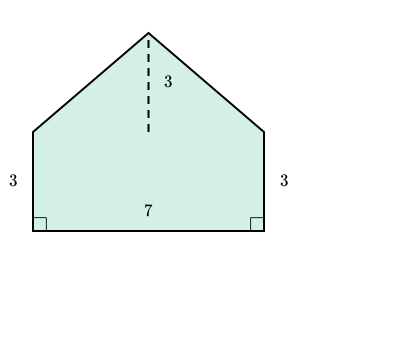
\includegraphics[scale=\shrinkfactor]{figures/2e4ce4191b4fc38f257d0fa2cf77a91ef947d85e.png}

\paragraph{Ans}  [[? input-number 1]] $\text{in}^2$  189

\paragraph{Hint 1}This shape is made up of a rectangle with a triangle on the top.   


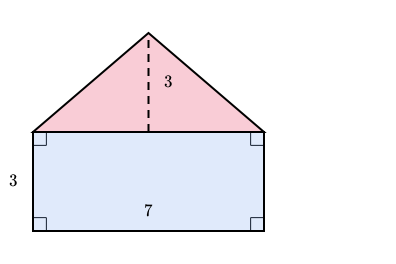
\includegraphics[scale=\shrinkfactor]{figures/31c1e6aea80c6123a5e9b4a17051aa39258832da.png}  

We know the rectangle is $7$ inches long and $3$ inches wide.  

$\blue{\text{Area}}=\blue7\cdot\blue3=21\text{ in}^2$  

The triangle on the top can be divided into two right triangles and then combined to form a rectangle.  


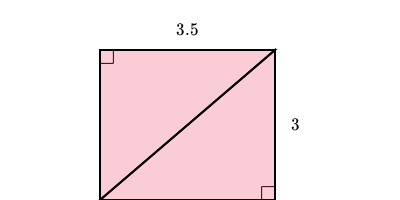
\includegraphics[scale=\shrinkfactor]{figures/9599530e43ce1e412d40dc6e75c5789216f0dac5.png}  
  
$\red{\text{Area}}=\red3\red.\red5\cdot\red3=10.5\text{ in}^2$

\paragraph{Hint 2}To find the total area of the shape, we can combine the two areas we found:  

$\blue2\blue1+\red1\red0\red.\red5=\green3\green1\green.\green5$  

\paragraph{Hint 3}The area of one figure is $\green3\green1\green.\green5$ square inches.
We need $\purple6$ of these figures.

$\green3\green1\green.\green5\cdot\purple6=189\text{ in}^2$

\paragraph{Hint 4}The area of the figure is $189\text{ in}^2$



\medskip
\noindent
\textbf{Tags:} {\footnotesize CC.6.G.A.1, i.	Composing and Decomposing Shapes 1.1, SB.6.1.H.1.CR}\\
\textbf{Version:} f3a2ecde.. 2013-10-06
\smallskip\hrule





\section{\href{https://www.khanacademy.org/devadmin/content/items/x1c6e2f705d8cdae4}{x1c6e2f705d8cdae4}}

\noindent
Tom and Jerry have a wrestling ring in their backyard.  Their ring is an octagon- an eight sided figure- enclosed in a square fence.  In the drawing below, the sides are in feet.  **What is the area of the octagon?**


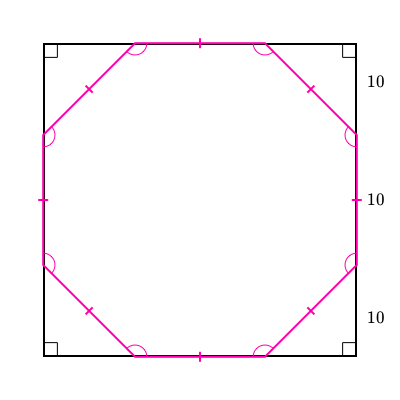
\includegraphics[scale=\shrinkfactor]{figures/dbc27f28399165541bacc602846575cddbd21659.png}

\paragraph{Ans}  [[? input-number 1]] $\text{ft}^2$  700

\paragraph{Hint 1}We know the square is $30$ feet long and $30$ feet wide.  
${\text{Area}}=30\cdot30=900\text{ ft}^2$  

\paragraph{Hint 2}We have 4 right triangles that are the same size and shape.  

We can combine two right triangles to form another square: 


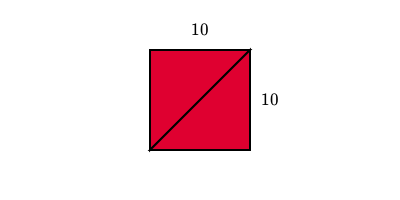
\includegraphics[scale=\shrinkfactor]{figures/7b202092b90108ba9707f033da2930445cb57204.png}      

${\text{Area}}=10\cdot10=100\text{ ft}^2$  

Since we have $2$ more triangles, we can make another square, so we need to multiply the area of this square by $2$.  

$2\cdot100=200\text{ ft}^2$

The area of the four triangles combined is $200\text{ ft}^2$.

\paragraph{Hint 3}If we subtract the combined area of the triangles from the area of the square, we will find the area of the octagon.  

$900\text{ ft}^2-200\text{ ft}^2=700\text{ ft}^2$

\paragraph{Hint 4}The area of the octagon is $700\text{ ft}^2$.



\medskip
\noindent
\textbf{Tags:} {\footnotesize CC.6.G.A.1, i.	Composing and Decomposing Shapes 1.1, SB.6.1.H.1.CR}\\
\textbf{Version:} 3131a505.. 2013-10-07
\smallskip\hrule





\section{\href{https://www.khanacademy.org/devadmin/content/items/x3748626441dc2c4c}{x3748626441dc2c4c}}

\noindent
Carl is making a poster for a pep rally.  He needs to create $8$ figures exactly the same size and shape as the figure below, which is measured in inches.  
 
**How many square inches of paper will his figures measure in total?**  


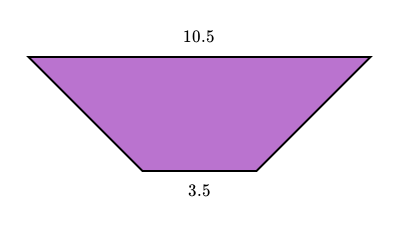
\includegraphics[scale=\shrinkfactor]{figures/06f69a34ae9e542486f5a6ed56b58449dfc9484d.png}

\paragraph{Ans}  [[? input-number 1]] $\text{in}^2$  100

\paragraph{Hint 1}This shape is made up of a square at the center and two right triangles on the sides.   

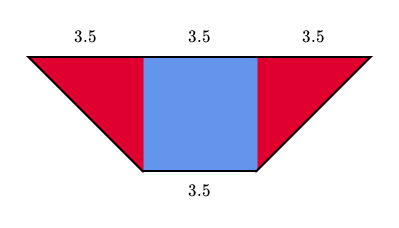
\includegraphics[scale=\shrinkfactor]{figures/69e2aa82ce5a56c3f084d88e1071a8d88082f00d.png}    
We know the base of the shape is $3.5$ inches wide, so we can form a square at the center of the shape with side length $3.5$ inches.

$\blue{\text{Area}}=\blue3\blue.\blue5\cdot\blue3\blue.\blue5=12.25\text{ in}^2$

We can combine the two right triangles to form another square:  


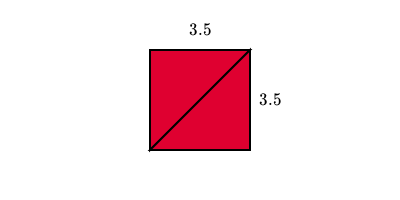
\includegraphics[scale=\shrinkfactor]{figures/18103602f712848d464d02c372e805b37743cbb8.png}    
  
$\red{\text{Area}}=\red3\red.\red5\cdot\red3\red.\red5=12.25\text{ in}^2$

\paragraph{Hint 2}To find the total area of the shape, we can combine the two areas we found:  

$\blue1\blue2\blue.\blue2\blue5+\red1\red2\red.\red2\red5=\purple2\purple4\purple.\purple5$  

The area of one figure is $\purple2\purple4\purple.\purple5$ square inches.
We need $\green8$ of these figures for the poster.

$\purple2\purple4\purple.\purple5\cdot\green8=100\text{ in}^2$

\paragraph{Hint 3}The figures will measure $100$ $\text{ in}^2$ in total.



\medskip
\noindent
\textbf{Tags:} {\footnotesize CC.6.G.A.1, i.	Composing and Decomposing Shapes 1.1, SB.6.1.H.1.CR}\\
\textbf{Version:} d522a540.. 2013-10-10
\smallskip\hrule





\section{\href{https://www.khanacademy.org/devadmin/content/items/x3bba6b5c4863bda7}{x3bba6b5c4863bda7}}

\noindent
Phyllis is making a metal sign for her yard.  She needs to create $10$ figures exactly the same size and shape as the figure below, which is measured in inches.   

**How many square inches of metal will her figures measure in total?**  


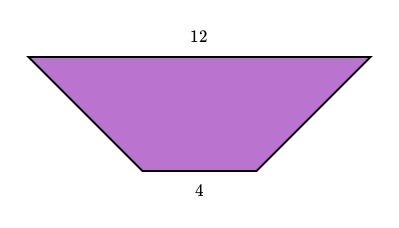
\includegraphics[scale=\shrinkfactor]{figures/91f52fa6e7dc99094c665735d3ea81069a5ed0bc.png}

\paragraph{Ans}  [[? input-number 1]] $\text{in}^2$  320

\paragraph{Hint 1}This shape is made up of a square at the center and two right triangles on the sides.   

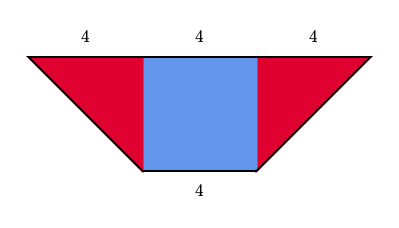
\includegraphics[scale=\shrinkfactor]{figures/a4b367a438e14d33c4a60e14958ce9494144a04b.png}   
We know the base of the shape is $4$ inches wide, so we can form a square at the center of the shape with side length $4$ inches.

$\blue{\text{Area}}=\blue4\cdot\blue4=16\text{ in}^2$

We can combine the two right triangles to form another square:  


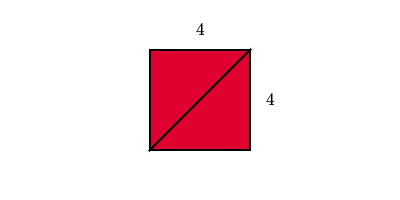
\includegraphics[scale=\shrinkfactor]{figures/36f7428d3898321b87f0422b6826d376709933ab.png}      
  
$\red{\text{Area}}=\red4\cdot\red4=16\text{ in}^2$

\paragraph{Hint 2}To find the total area of the shape, we can combine the two areas we found:  

$\blue1\blue6+\red1\red6=\purple3\purple2$  

The area of one figure is $\purple3\purple2$ square inches.
We need $\green1\green0$ of these figures for the sign.

$\purple3\purple2\cdot\green1\green0=320\text{ in}^2$

\paragraph{Hint 3}The figures will measure $320$ $\text{ in}^2$ in total.



\medskip
\noindent
\textbf{Tags:} {\footnotesize CC.6.G.A.1, i.	Composing and Decomposing Shapes 1.1, SB.6.1.H.1.CR}\\
\textbf{Version:} 77411c26.. 2013-10-10
\smallskip\hrule





\section{\href{https://www.khanacademy.org/devadmin/content/items/x405cd06e1a64fe0a}{x405cd06e1a64fe0a}}

\noindent
Amy's family loves the Broncos, so she is going to make them flags to hang on their porches.  She is going to create $20$ flags exactly the same size and shape as the figure below, which is measured in feet.  

**How many square feet of fabric will Amy's figures measure in total?**  


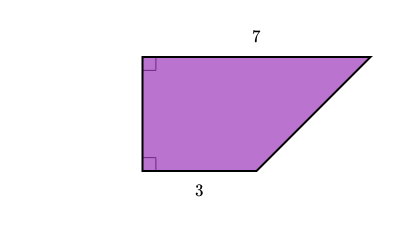
\includegraphics[scale=\shrinkfactor]{figures/cb61a5432b8e6593a6d5b9cee1d0b469d333ffb8.png}

\paragraph{Ans}  [[? input-number 1]] $\text{ft}^2$  340

\paragraph{Hint 1}This shape is made up of a square with a right triangle on the side.   

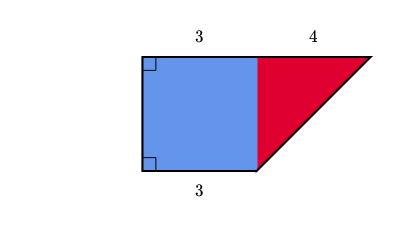
\includegraphics[scale=\shrinkfactor]{figures/067cc5d1e80218ad8d46b5aa2299faedad10693e.png}      
We know the base of the shape is $3$ feet wide, so we can form a square with side length $3$ feet.

$\blue{\text{Area}}=\blue3\cdot\blue3=9\text{ ft}^2$

The right triangle on the side is one half of another square:


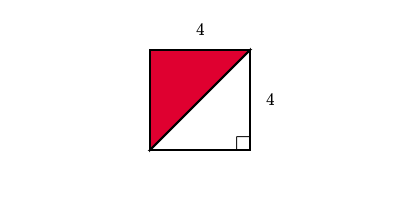
\includegraphics[scale=\shrinkfactor]{figures/51d21298447de315e7267fbd46031e5724227ff0.png}     
  
$\red{\text{Area}}=\dfrac{1}{2}\cdot\red4\cdot\red4=\dfrac{1}{2}\cdot16\text{ ft}^2=8\text{ ft}^2$

\paragraph{Hint 2}To find the total area of the shape, we can combine the two areas we found:  

$\blue9+\red8=\purple1\purple7$  

The area of one figure is $\purple1\purple7$ square feet.  
Amy is making $\green2\green0$ of these figures for the flags.

$\purple1\purple7\cdot\green2\green0=340\text{ ft}^2$

\paragraph{Hint 3}The figures will measure $340\text{ ft}^2$ in total.



\medskip
\noindent
\textbf{Tags:} {\footnotesize CC.6.G.A.1, i.	Composing and Decomposing Shapes 1.1, SB.6.1.H.1.CR}\\
\textbf{Version:} c3444470.. 2013-10-09
\smallskip\hrule





\section{\href{https://www.khanacademy.org/devadmin/content/items/x4aa3a7d56645732b}{x4aa3a7d56645732b}}

\noindent
Terry's family is going on a trip to a Saints football game, and they are making matching car flags for their vehicles.  He is going to create $8$ flags exactly the same size and shape as the figure below, which is measured in inches.  

**How many square inches of fabric will Terry's figures measure in total?**  


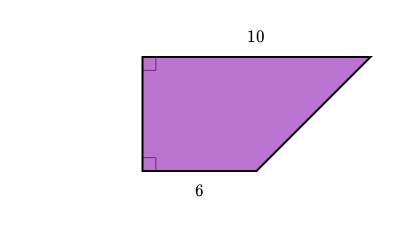
\includegraphics[scale=\shrinkfactor]{figures/0ec9c736dcaf37f09c67ea2ca5c67ba0166e472a.png}

\paragraph{Ans}  [[? input-number 1]] $\text{in}^2$  352

\paragraph{Hint 1}This shape is made up of a square with a right triangle on the side.   

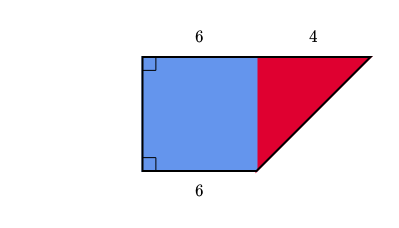
\includegraphics[scale=\shrinkfactor]{figures/99e259fa022bc41c81451597b8921af6b683f739.png}    
We know the base of the shape is $6$ inches wide, so we can form a square with side length $6$ inches.

$\blue{\text{Area}}=\blue6\cdot\blue6=36\text{ in}^2$

The right triangle on the side is one half of another square:


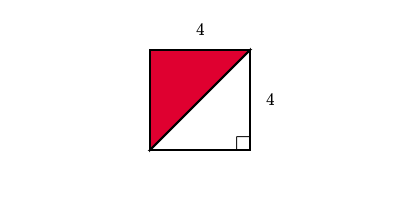
\includegraphics[scale=\shrinkfactor]{figures/51d21298447de315e7267fbd46031e5724227ff0.png}     
  
$\red{\text{Area}}=\dfrac{1}{2}\cdot\red4\cdot\red4=\dfrac{1}{2}\cdot16\text{ in}^2=8\text{ in}^2$

\paragraph{Hint 2}To find the total area of the shape, we can combine the two areas we found:  

$\blue3\blue6+\red8=\purple4\purple4$  

The area of one figure is $\purple4\purple4$ square inches.
Terry is making $\green8$ of these figures for the flags.

$\purple4\purple4\cdot\green8=352\text{ in}^2$

\paragraph{Hint 3}The figures will measure $352\text{ in}^2$ in total.



\medskip
\noindent
\textbf{Tags:} {\footnotesize CC.6.G.A.1, i.	Composing and Decomposing Shapes 1.1, SB.6.1.H.1.CR}\\
\textbf{Version:} 95de722e.. 2013-10-09
\smallskip\hrule





\section{\href{https://www.khanacademy.org/devadmin/content/items/x4c1b6ee09e08a9a0}{x4c1b6ee09e08a9a0}}

\noindent
Mrs. LeJeune is decorating her bulletin board.  She is covering the board with paper and then placing a border along each edge of the board.  **Using the picture below, what is the area of the border if the dimensions are in feet?**  


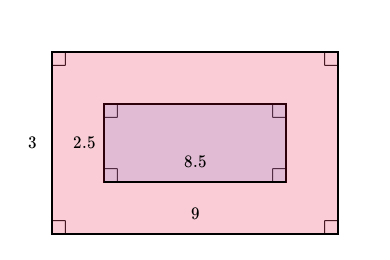
\includegraphics[scale=\shrinkfactor]{figures/c7954a5c36472e222f1bd6e7e53e5059a4a1b23a.png}

\paragraph{Ans}  [[? input-number 1]] $\text{ft}^2$  5.75

\paragraph{Hint 1}First, we need to find the area of the entire rectangle.  


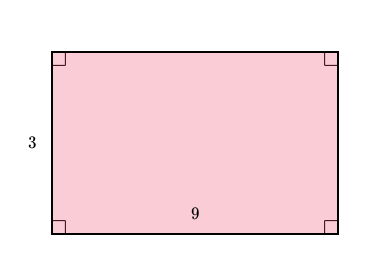
\includegraphics[scale=\shrinkfactor]{figures/64da7088e42aa9dca888583ead3d7b5ca4760ea9.png}    
 
$Area=9\times3=27  \text{ ft}^2$  

\paragraph{Hint 2}Then we find the area of the rectangle on the inside.  


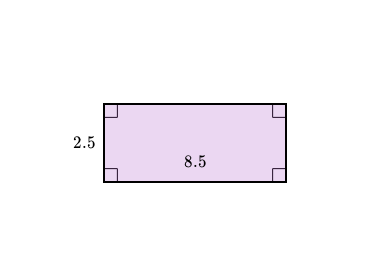
\includegraphics[scale=\shrinkfactor]{figures/37cac3066659606b57259837537cc3ba672dcc2a.png}  

$Area=8.5\times2.5=21.25  \text{ ft}^2$  

\paragraph{Hint 3}We can find the area of the border by finding the area of the larger rectangle and subtracting the area of the smaller rectangle. 

$27-21.25=5.75\text{ ft}^2$ 

\paragraph{Hint 4}The area of the border is $5.75\text{ ft}^2$ 



\medskip
\noindent
\textbf{Tags:} {\footnotesize CC.6.G.A.1, i.	Composing and Decomposing Shapes 1.1, SB.6.1.H.1.CR}\\
\textbf{Version:} a7ad974b.. 2013-10-07
\smallskip\hrule





\section{\href{https://www.khanacademy.org/devadmin/content/items/x4c306a907c3d7c75}{x4c306a907c3d7c75}}

\noindent
Boudreaux High School is selling porch flags to support their basketball team.  The school is going to create $150$ flags exactly the same size and shape as the figure below, which is measured in feet.  

**How many square feet of fabric will Boudreaux High School's figures measure in total?**  


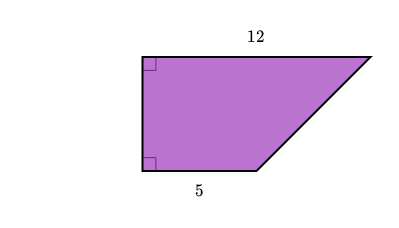
\includegraphics[scale=\shrinkfactor]{figures/0e7c700411f05668463e1f8fba31ed97ab7090cd.png}

\paragraph{Ans}  [[? input-number 1]] $\text{ft}^2$  7425

\paragraph{Hint 1}This shape is made up of a square with a right triangle on the side.   

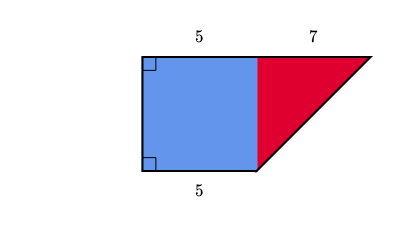
\includegraphics[scale=\shrinkfactor]{figures/f9c9cacd311053dfbda35f01755b43e40d00a74e.png}        
We know the base of the shape is $5$ feet wide, so we can form a square with side length $5$ feet.

$\blue{\text{Area}}=\blue5\cdot\blue5=25\text{ ft}^2$

The right triangle on the side is one half of another square:


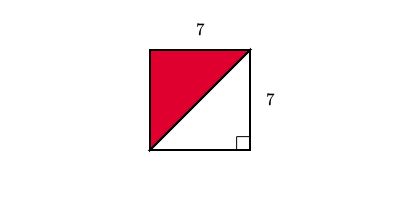
\includegraphics[scale=\shrinkfactor]{figures/ec74e4bed20caece7a1fa1e9967f65010ff22993.png}       
  
$\red{\text{Area}}=\dfrac{1}{2}\cdot\red7\cdot\red7=\dfrac{1}{2}\cdot49\text{ ft}^2=24.5\text{ ft}^2$

\paragraph{Hint 2}To find the total area of the shape, we can combine the two areas we found:  

$\blue2\blue5+\red2\red4\red.\red5=\purple4\purple9\purple.\purple5  $

The area of one figure is $\purple4\purple9\purple.\purple5$ square feet.  
Boudreaux High School is making $\green1\green5\green0$ of these figures for the flags.

$\purple4\purple9\purple.\purple5\cdot\green1\green5\green0=7425\text{ ft}^2$

\paragraph{Hint 3}The figures will measure $7425\text{ ft}^2$ in total.



\medskip
\noindent
\textbf{Tags:} {\footnotesize CC.6.G.A.1, i.	Composing and Decomposing Shapes 1.1, SB.6.1.H.1.CR}\\
\textbf{Version:} d50ac771.. 2013-10-09
\smallskip\hrule





\section{\href{https://www.khanacademy.org/devadmin/content/items/x5b75eef1a7151a83}{x5b75eef1a7151a83}}

\noindent
Annie is painting a wall.  The picture below, which is measured in feet, represents the area that she has painted so far.    

**How many square feet of wall has Annie painted?**  


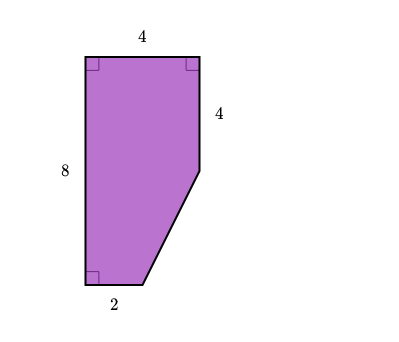
\includegraphics[scale=\shrinkfactor]{figures/ed8d325b95059dd0c8803395e12520bc9ff14cd4.png}

\paragraph{Ans}  [[? input-number 1]] $\text{feet}^2$  28

\paragraph{Hint 1}This shape is made up of a square at the top, a rectangle on the left side, and a triangle on the right side.    


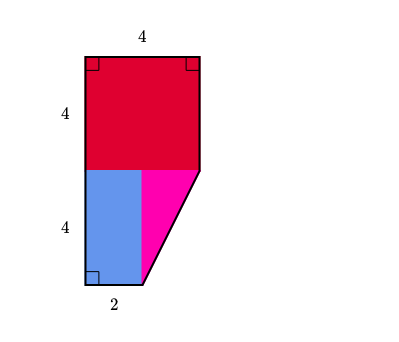
\includegraphics[scale=\shrinkfactor]{figures/b38c10de64f86ab72f10f002bed91ecdbb4d02ab.png}  
 
We know the square at the top of the shape has a side length of $4$ feet.

$\red{\text{Area}}=\red4\cdot\red4=16\text{ feet}^2$


We know the rectangle on the left side has a length of $4$ feet and a width of $2$ feet.   

$\blue{\text{Area}}=\blue4\cdot\blue2=8\text{ feet}^2$  

The triangle on the right side is one-half of another rectangle:  


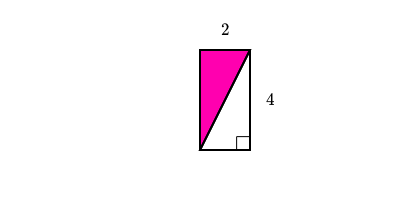
\includegraphics[scale=\shrinkfactor]{figures/9de1df5c9528633fa1c1d6d960e6653431c488cc.png}  

$\pink{\text{Area}}=\dfrac{1}{2}\cdot\pink4\cdot\pink2=\dfrac{1}{2}\cdot8\text{ feet}^2=4\text{ feet}^2$

\paragraph{Hint 2}To find the total area of the shape, we can combine the three areas we found:  

$\red1\red6+\blue8+\pink4=\purple2\purple8$  

The area of this figure is $\purple2\purple8$ square feet.  

\paragraph{Hint 3}Annie has painted $28$ $\text{ feet}^2$ in total.



\medskip
\noindent
\textbf{Tags:} {\footnotesize CC.6.G.A.1, i.	Composing and Decomposing Shapes 1.1, SB.6.1.H.1.CR}\\
\textbf{Version:} 476595a3.. 2013-10-11
\smallskip\hrule





\section{\href{https://www.khanacademy.org/devadmin/content/items/x5dc8c670f44d1837}{x5dc8c670f44d1837}}

\noindent
Blaine is painting a design on a wall.  The picture below, which is measured in inches, represents one of the shapes that he is painting on the wall.  

**If Blaine painted 22 of these figures on the wall, how many square feet of wall has Blaine painted?**  


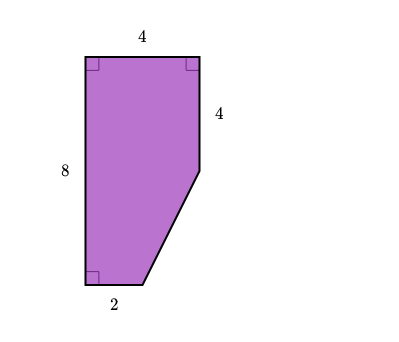
\includegraphics[scale=\shrinkfactor]{figures/ed8d325b95059dd0c8803395e12520bc9ff14cd4.png}

\paragraph{Ans}  [[? input-number 1]] $\text{feet}^2$  616

\paragraph{Hint 1}This shape is made up of a square at the top, a rectangle on the left side, and a triangle on the right side.    


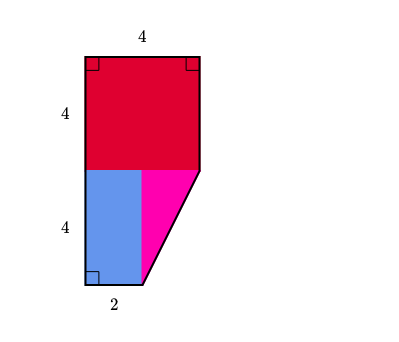
\includegraphics[scale=\shrinkfactor]{figures/b38c10de64f86ab72f10f002bed91ecdbb4d02ab.png}  
 
We know the square at the top of the shape has a side length of $4$ inches.

$\red{\text{Area}}=\red4\cdot\red4=16\text{ inches}^2$


We know the rectangle on the left side has a length of $4$ inches and a width of $2$ inches.   

$\blue{\text{Area}}=\blue4\cdot\blue2=8\text{ inches}^2$  

The triangle on the right side is one-half of another rectangle:  


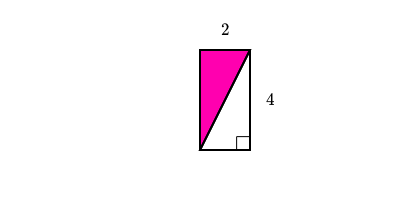
\includegraphics[scale=\shrinkfactor]{figures/9de1df5c9528633fa1c1d6d960e6653431c488cc.png}  

$\pink{\text{Area}}=\dfrac{1}{2}\cdot\pink4\cdot\pink2=\dfrac{1}{2}\cdot8\text{ inches}^2=4\text{ inches}^2$

\paragraph{Hint 2}To find the total area of the shape, we can combine the three areas we found:  

$\red1\red6+\blue8+\pink4=\purple2\purple8$  

The area of this figure is $\purple2\purple8$ square feet.  



\paragraph{Hint 3}The area of one figure is $\green2\green8$ square inches.
We need $\purple2\purple2$ of these figures.

$\green2\green8\cdot\purple2\purple2=616\text{ in}^2$

\paragraph{Hint 4}Blaine has painted $616$ $\text{ inches}^2$ in total.



\medskip
\noindent
\textbf{Tags:} {\footnotesize CC.6.G.A.1, i.	Composing and Decomposing Shapes 1.1, SB.6.1.H.1.CR}\\
\textbf{Version:} 3e78374a.. 2013-10-11
\smallskip\hrule





\section{\href{https://www.khanacademy.org/devadmin/content/items/x6457d5067a42fab1}{x6457d5067a42fab1}}

\noindent
Tracey is working on her graduation scrapbook.  She cut the corners off of a square picture in order to create an octagon- an eight sided figure.  In the drawing below, the sides are in inches.  **What is the area of the trimmed picture?**  


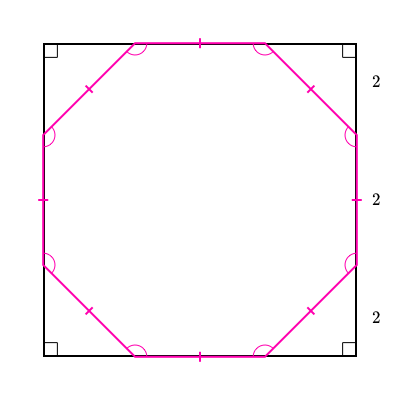
\includegraphics[scale=\shrinkfactor]{figures/594b710dd149095c7310e73a8ff73437fd084a77.png}

\paragraph{Ans}  [[? input-number 1]] $\text{in}^2$  56

\paragraph{Hint 1}We know the original square picture is $8$ inches long and $8$ inches wide.  
${\text{Area}}=8\cdot8=64\text{ in}^2$  

\paragraph{Hint 2}We have 4 right triangles that are the same size and shape.  

We can combine two right triangles to form another square: 


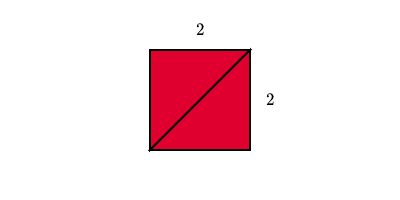
\includegraphics[scale=\shrinkfactor]{figures/8990031770cbd0af85eeed620a6be4bcc4e04b7b.png}      

${\text{Area}}=2\cdot2=4\text{ in}^2$  

Since we have $2$ more triangles, we can make another square, so we need to multiply the area of this square by $2$.  

$2\cdot4=8\text{ in}^2$

The area of the four triangles combined is $8\text{ in}^2$.

\paragraph{Hint 3}If we subtract the combined area of the triangles from the area of the square, we will find the area of the trimmed picture.  

$64\text{ in}^2-8\text{ in}^2=56\text{ in}^2$

\paragraph{Hint 4}The area of the trimmed picture is $56\text{ in}^2$.



\medskip
\noindent
\textbf{Tags:} {\footnotesize CC.6.G.A.1, i.	Composing and Decomposing Shapes 1.1, SB.6.1.H.1.CR}\\
\textbf{Version:} d7db7c47.. 2013-10-07
\smallskip\hrule





\section{\href{https://www.khanacademy.org/devadmin/content/items/x6e3f6cd12498db47}{x6e3f6cd12498db47}}

\noindent
Buffy and her sister Dawn have a 10 feet by 40 feet rectangular lap pool in their backyard.  They are not getting along today, so they are going to divide the pool in half diagonally with a rope.  **What is the area of the swimming pool that each of them will have if the sides are measured in feet?**  

\paragraph{Ans}  [[? input-number 1]] $\text{ft}^2$  200

\paragraph{Hint 1}First let's draw a model of our swimming pool.  


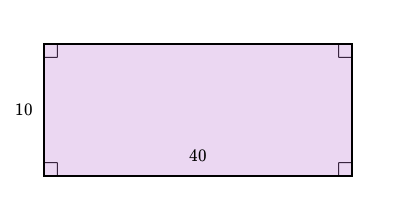
\includegraphics[scale=\shrinkfactor]{figures/19902d36cb6bfded708f436f2951427d0b173e94.png}  

We know the rectangle is $40$ feet long and $10$ feet wide.  
${\text{Area}}=40\cdot10=400\text{ ft}^2$  

\paragraph{Hint 2}They are going to divide the pool in half.  

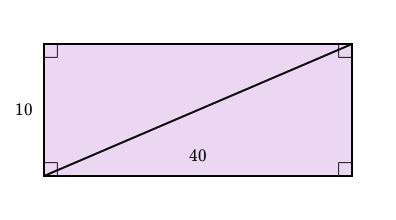
\includegraphics[scale=\shrinkfactor]{figures/2f77060cc398289e1491af1f812dcd21706f3116.png}  

We need to figure out half of the area of the entire rectangle.    

${\text{Area}}=\dfrac{1}{2}\cdot400=200\text{ ft}^2$  

\paragraph{Hint 3}The area of half of the pool is $200\text{ ft}^2$.



\medskip
\noindent
\textbf{Tags:} {\footnotesize CC.6.G.A.1, i.	Composing and Decomposing Shapes 1.1, SB.6.1.H.1.CR}\\
\textbf{Version:} d94b226e.. 2013-10-07
\smallskip\hrule





\section{\href{https://www.khanacademy.org/devadmin/content/items/x793958e5c731dffd}{x793958e5c731dffd}}

\noindent
Olivia is cutting an $8.5\text{ inch}$ by $11\text{ inch}$ piece of paper diagonally.  **What is the area of each piece after she makes her cut?**  

\paragraph{Ans}  [[? input-number 1]] $\text{in}^2$  46.75

\paragraph{Hint 1}First let's draw a model of our swimming pool.  


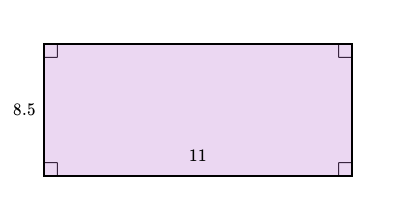
\includegraphics[scale=\shrinkfactor]{figures/8a2c3ed0982713da37ab82c1f45c53d7c8168214.png}    

We know the rectangle is $11$ inch long and $8.5$ inch wide.  
${\text{Area}}=11\cdot8.5=93.5\text{ in}^2$  

\paragraph{Hint 2}She is going to cut the paper in half.  


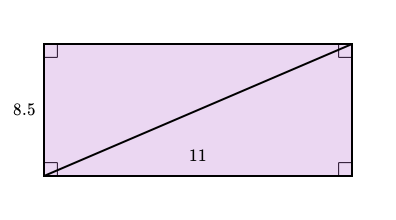
\includegraphics[scale=\shrinkfactor]{figures/7c2af295e1180eb4e39fbbd8921bcd930561a85b.png}  

We need to figure out half of the area of the entire rectangle.    

${\text{Area}}=\dfrac{1}{2}\cdot93.5=46.75\text{ in}^2$  

\paragraph{Hint 3}The area of half of the paper is $46.75\text{ in}^2$.



\medskip
\noindent
\textbf{Tags:} {\footnotesize CC.6.G.A.1, i.	Composing and Decomposing Shapes 1.1, SB.6.1.H.1.CR}\\
\textbf{Version:} 2c1d451e.. 2013-10-07
\smallskip\hrule





\section{\href{https://www.khanacademy.org/devadmin/content/items/x80c83b209703765e}{x80c83b209703765e}}

\noindent
You were just elected president of the Student Council at your school.  Now you are responsible for decorating the bulletin board in the hall outside of the office.  You need to create $5$ figures exactly the same size and shape as the figure below, which is measured in inches.  

**How many square inches of paper will your figures measure in total?**  


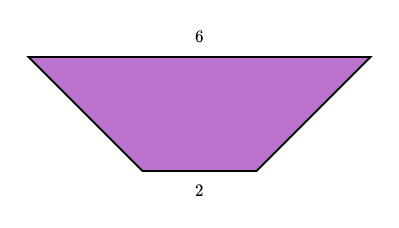
\includegraphics[scale=\shrinkfactor]{figures/781cdfbe1757418bfa130d321768939d3b1a9f15.png}  

\paragraph{Ans}  [[? input-number 1]] $\text{in}^2$  40

\paragraph{Hint 1}This shape is made up of a square at the center and two right triangles on the sides.   

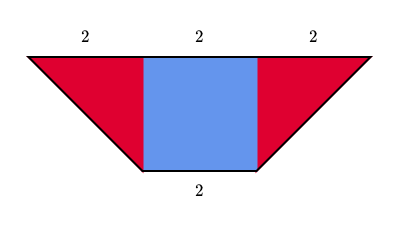
\includegraphics[scale=\shrinkfactor]{figures/3f4ee8f5688926d984784cd27641388192134f32.png}  
We know the base of the shape is $2$ inches wide, so we can form a square at the center of the shape with side length $2$ inches.

$\blue{\text{Area}}=\blue2\cdot\blue2=4\text{ in}^2$

We can combine the two right triangles to form another square:

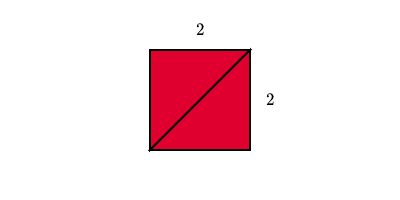
\includegraphics[scale=\shrinkfactor]{figures/8990031770cbd0af85eeed620a6be4bcc4e04b7b.png}  
  
$\red{\text{Area}}=\red2\cdot\red2=4\text{ in}^2$

\paragraph{Hint 2}To find the total area of the shape, we can combine the two areas we found:  

$\blue4+\red4=\purple8$  

The area of one figure is $\purple8$ square inches.
We need $\green5$ of these figures for the bulletin board.

$\purple8\cdot\green5=40\text{ in}^2$

\paragraph{Hint 3}The figures will measure $40$ $\text{ in}^2$ in total.



\medskip
\noindent
\textbf{Tags:} {\footnotesize CC.6.G.A.1, i.	Composing and Decomposing Shapes 1.1, SB.6.1.H.1.CR}\\
\textbf{Version:} 665e26eb.. 2013-10-06
\smallskip\hrule





\section{\href{https://www.khanacademy.org/devadmin/content/items/x8247cfe2962a2672}{x8247cfe2962a2672}}

\noindent
Barney is putting a picture in a frame.  **Using the picture below, what is the area of the frame if the dimensions are in inches?**  


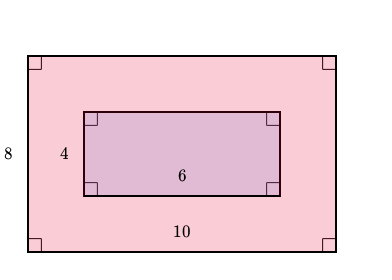
\includegraphics[scale=\shrinkfactor]{figures/4546e6b0eb1441ca90cd9bf45ec19a52472daab2.png}

\paragraph{Ans}  [[? input-number 1]] $\text{in}^2$  56

\paragraph{Hint 1}First, we need to find the area of the entire rectangle.  


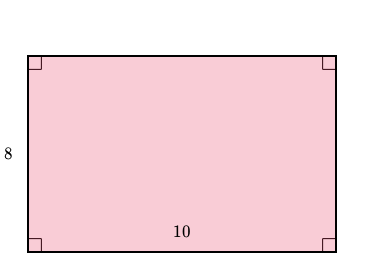
\includegraphics[scale=\shrinkfactor]{figures/840752dfa9d7f16638349beb8996e329917ecac4.png}
 
$Area=10\times8=80  \text{ in}^2$  

\paragraph{Hint 2}Then we find the area of the rectangle on the inside.  


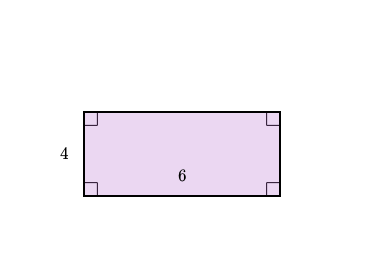
\includegraphics[scale=\shrinkfactor]{figures/a7b048032baf0298ab335931877732a0a2bc0db5.png}  

$Area=6\times4=24  \text{ in}^2$  

\paragraph{Hint 3}We can find the area of the frame by finding the area of the larger rectangle and subtracting the area of the smaller rectangle. 

$80-24=56\text{ in}^2$ 

\paragraph{Hint 4}The area of the frame is $56\text{ in}^2$ 



\medskip
\noindent
\textbf{Tags:} {\footnotesize CC.6.G.A.1, i.	Composing and Decomposing Shapes 1.1, SB.6.1.H.1.CR}\\
\textbf{Version:} 81a410fb.. 2013-10-07
\smallskip\hrule





\section{\href{https://www.khanacademy.org/devadmin/content/items/x83417cfed56951cb}{x83417cfed56951cb}}

\noindent
Amy is captain of the cheerleading squad at her school, and her school's football team is going to the state championships!  To support the team, the cheerleading squad is selling car flags.  She is going to create $50$ flags exactly the same size and shape as the figure below, which is measured in inches.  

**How many square inches of fabric will Amy's figures measure in total?**  


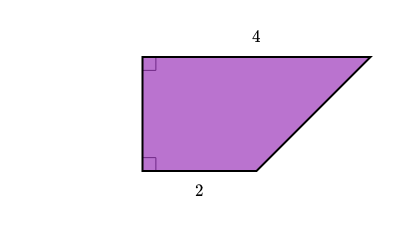
\includegraphics[scale=\shrinkfactor]{figures/05e73ba50508f13e74a3e721f9928d037170ce23.png}

\paragraph{Ans}  [[? input-number 1]] $\text{in}^2$  300

\paragraph{Hint 1}This shape is made up of a square with a right triangle on the side.   

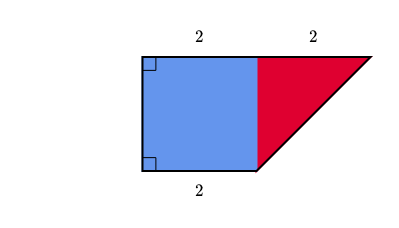
\includegraphics[scale=\shrinkfactor]{figures/fc70c0d8454a16c4a307830817a98559cbc90e2c.png}  
We know the base of the shape is $2$ inches wide, so we can form a square with side length $2$ inches.

$\blue{\text{Area}}=\blue2\cdot\blue2=4\text{ in}^2$

The right triangle on the side is one half of another square:


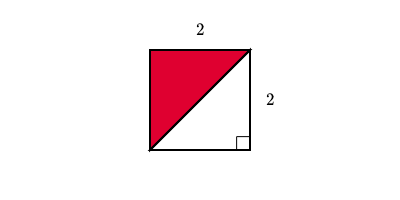
\includegraphics[scale=\shrinkfactor]{figures/fb8af8a0de7d7859fb2dd9cfa4dfb6a1f0b39275.png}    
  
$\red{\text{Area}}=\dfrac{1}{2}\cdot\red2\cdot\red2=\dfrac{1}{2}\cdot4\text{ in}^2=2\text{ in}^2$

\paragraph{Hint 2}To find the total area of the shape, we can combine the two areas we found:  

$\blue4+\red2=\purple6$  

The area of one figure is $\purple6$ square inches.
Amy is making $\green5\green0$ of these figures for the flags.

$\purple6\cdot\green5\green0=300\text{ in}^2$

\paragraph{Hint 3}The figures will measure $300\text{ in}^2$ in total.



\medskip
\noindent
\textbf{Tags:} {\footnotesize CC.6.G.A.1, i.	Composing and Decomposing Shapes 1.1, SB.6.1.H.1.CR}\\
\textbf{Version:} 4e7b7ede.. 2013-09-30
\smallskip\hrule





\section{\href{https://www.khanacademy.org/devadmin/content/items/x8c6bc6e1d75edb7d}{x8c6bc6e1d75edb7d}}

\noindent
Lonnie is painting his bathroom.  The picture below, which is measured in feet, represents the area that he has painted so far.    

**How many square feet of wall has Lonnie painted?**  


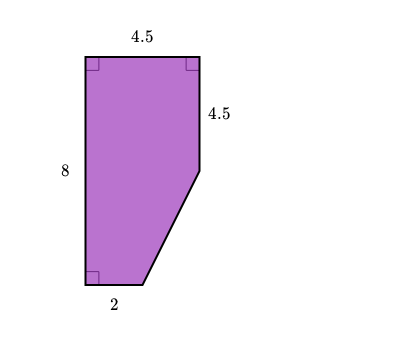
\includegraphics[scale=\shrinkfactor]{figures/d7a4685e7788c0e227f7aaf8e965683173e51a3d.png}

\paragraph{Ans}  [[? input-number 1]] $\text{feet}^2$  32.0625

\paragraph{Hint 1}This shape is made up of a square at the top, a rectangle on the left side, and a triangle on the right side.    


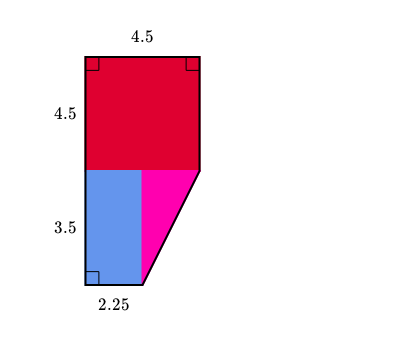
\includegraphics[scale=\shrinkfactor]{figures/8899f8ff2cb9fc95c67126eaaa7af49d01cad2df.png}  
 
We know the square at the top of the shape has a side length of $4.5$ feet.

$\red{\text{Area}}=\red4\red.\red5\cdot\red4\red.\red5=20.25\text{ feet}^2$


We know the rectangle on the left side has a length of $3.5$ feet and a width of $2.25$ feet.   

$\blue{\text{Area}}=\blue3\blue.\blue5\cdot\blue2\blue.\blue2\blue5=7.875\text{ feet}^2$  

The triangle on the right side is one-half of another rectangle:  


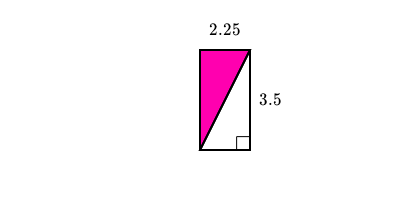
\includegraphics[scale=\shrinkfactor]{figures/ab4b2b7901fd06eb31f3170da5448710f69c25f1.png}  

$\pink{\text{Area}}=\dfrac{1}{2}\cdot\pink3\pink.\pink5\cdot\pink2\pink.\pink2\pink5=\dfrac{1}{2}\cdot7.875\text{ feet}^2=3.9375\text{ feet}^2$

\paragraph{Hint 2}To find the total area of the shape, we can combine the three areas we found:  

$\red2\red0\red.\red2\red5+\blue7\blue.\blue8\blue7\blue5+\pink3\pink.\pink9\pink3\pink7\pink5=\purple2\purple8$  

The area of this figure is $\purple3\purple2\purple.\purple0\purple6\purple2\purple5$ square feet.  

\paragraph{Hint 3}Annie has painted $32.0625$ $\text{ feet}^2$ in total.



\medskip
\noindent
\textbf{Tags:} {\footnotesize CC.6.G.A.1, i.	Composing and Decomposing Shapes 1.1, SB.6.1.H.1.CR}\\
\textbf{Version:} 23dfcc7c.. 2013-10-11
\smallskip\hrule





\section{\href{https://www.khanacademy.org/devadmin/content/items/x9c5a0a3921162972}{x9c5a0a3921162972}}

\noindent
Bethany is cutting the grass.  The picture below, which is measured in acres, represents the area that she has cut.    

**How many square acres of grass has Bethany cut?**  

\includegraphics[scale=\shrinkfactor]{figures/c98e616a3d3903e4dca17e8906756568108b880a.png}

\paragraph{Ans}  [[? input-number 1]] $\text{acres}^2$  7

\paragraph{Hint 1}This shape is made up of a square at the top, a rectangle on the left side, and a triangle on the right side.    


\includegraphics[scale=\shrinkfactor]{figures/0524e8c98a8595a05aa001bff09e60f738b9d254.png}  
 
We know the square at the top of the shape has a side length of $2$ acres.

$\red{\text{Area}}=\red2\cdot\red2=4\text{ acres}^2$


We know the rectangle on the left side has a length of $2$ acres and a width of $1$ acre.   

$\blue{\text{Area}}=\blue2\cdot\blue1=2\text{ acres}^2$  

The triangle on the right side is one-half of another rectangle:  



\includegraphics[scale=\shrinkfactor]{figures/06a39437df5105f36a7d54fd121f63d04c89e171.png}  

$\pink{\text{Area}}=\dfrac{1}{2}\cdot\pink2\cdot\pink1=\dfrac{1}{2}\cdot2\text{ acres}^2=1\text{ acres}^2$

\paragraph{Hint 2}To find the total area of the shape, we can combine the three areas we found:  

$\red4+\blue2+\pink1=\purple7$  

The area of this figure is $\purple7$ square acres.  

\paragraph{Hint 3}Bethany has cut $7$ $\text{ acres}^2$ in total.



\medskip
\noindent
\textbf{Tags:} {\footnotesize CC.6.G.A.1, i.	Composing and Decomposing Shapes 1.1, SB.6.1.H.1.CR}\\
\textbf{Version:} c0d90817.. 2013-10-11
\smallskip\hrule





\section{\href{https://www.khanacademy.org/devadmin/content/items/xa24b830a97fc8ae7}{xa24b830a97fc8ae7}}

\noindent
Jill has $10$ windows that she is going to cover with curtains.  **Using the model below, what is the area of the windows if the sides are measured in inches?**  


\includegraphics[scale=\shrinkfactor]{figures/276001c247b9c75560208dd3816091900a0cc4cd.png}

\paragraph{Ans}  [[? input-number 1]] $\text{in}^2$  2400

\paragraph{Hint 1}This shape is made up of a rectangle with a triangle on the top.   


\includegraphics[scale=\shrinkfactor]{figures/0c4023bececa3a58c09c109976f5e8ca813b7076.png}  

We know the rectangle is $20$ inches long and $10$ inches wide.  

$\green{\text{Area}}=\green2\green0\cdot\green1\green0=200\text{ in}^2$  

The triangle on the top can be divided into two right triangles and then combined to form a rectangle.  


\includegraphics[scale=\shrinkfactor]{figures/10b3b1d93ddc92e6db5268442e8fb7bfa030e91a.png}  
  
$\red{\text{Area}}=\red1\red0\cdot\red4=40\text{ in}^2$

\paragraph{Hint 2}To find the total area of the shape, we can combine the two areas we found:  

${\text{Area}}=\green2\green0\green0+\red4\red0=\purple2\purple4\purple0\text{ in}^2$

\paragraph{Hint 3}The area of one figure is $\green2\green4\green0$ square inches.
We need $\purple1\purple0$ of these figures.

$\green2\green4\green0\cdot\purple1\purple0=2400\text{ in}^2$

\paragraph{Hint 4}The area of the figure is $2400\text{ in}^2$



\medskip
\noindent
\textbf{Tags:} {\footnotesize CC.6.G.A.1, i.	Composing and Decomposing Shapes 1.1, SB.6.1.H.1.CR}\\
\textbf{Version:} efe15739.. 2013-10-06
\smallskip\hrule





\section{\href{https://www.khanacademy.org/devadmin/content/items/xb46775681091dd1e}{xb46775681091dd1e}}

\noindent
Bobby is decorating a rectangular cake.  He is going to put a rectangle of frosting around the border of the cake to form a smaller rectangle centered on the top of the cake.  **Using the picture below, what is the area of the icing border if the dimensions are in inches?**  


\includegraphics[scale=\shrinkfactor]{figures/9bc03a859f458109baa36d0d3443c45c898c9c5d.png}

\paragraph{Ans}  [[? input-number 1]] $\text{in}^2$  52

\paragraph{Hint 1}First, we need to find the area of the entire rectangle.  


\includegraphics[scale=\shrinkfactor]{figures/c78ac2659291464a5983a0bb8875175436f355d1.png}  
 
$Area=11\times17=187  \text{ in}^2$  

\paragraph{Hint 2}Then we find the area of the rectangle on the inside.  


\includegraphics[scale=\shrinkfactor]{figures/066ddfd1e947feed322c4fc9aec956edd50e9014.png}

$Area=15\times9=135  \text{ in}^2$  

\paragraph{Hint 3}We can find the area of the icing border by finding the area of the larger rectangle and subtracting the area of the smaller rectangle. 

$187-135=52\text{ in}^2$ 

\paragraph{Hint 4}The area of the icing border is $52\text{ in}^2$ 



\medskip
\noindent
\textbf{Tags:} {\footnotesize CC.6.G.A.1, i.	Composing and Decomposing Shapes 1.1, SB.6.1.H.1.CR}\\
\textbf{Version:} e8f05b5e.. 2013-10-07
\smallskip\hrule





\section{\href{https://www.khanacademy.org/devadmin/content/items/xcc05cd118a5fddc1}{xcc05cd118a5fddc1}}

\noindent
Jimmy is making a poster for his art class.  He needs to create $5$ figures exactly the same size and shape as the figure below, which is measured in inches.  
 
**How many square inches of paper will his figures measure in total?**  


\includegraphics[scale=\shrinkfactor]{figures/d8e846758f0427dfe7d64fa8f4fdad52e39d7b3c.png}

\paragraph{Ans}  [[? input-number 1]] $\text{in}^2$  62.5

\paragraph{Hint 1}This shape is made up of a square at the center and two right triangles on the sides.   

\includegraphics[scale=\shrinkfactor]{figures/2640748642b9d10d707ff53f18a61f2c577b3c60.png}  
We know the base of the shape is $2.5$ inches wide, so we can form a square at the center of the shape with side length $2.5$ inches.

$\blue{\text{Area}}=\blue2\blue.\blue5\cdot\blue2\blue.\blue5=6.25\text{ in}^2$

We can combine the two right triangles to form another square:  


\includegraphics[scale=\shrinkfactor]{figures/be1bc5772705af1eca32f8a77521f555510012fc.png}  
  
$\red{\text{Area}}=\red2\red.\red5\cdot\red2\red.\red5=6.25\text{ in}^2$

\paragraph{Hint 2}To find the total area of the shape, we can combine the two areas we found:  

$\blue6\blue.\blue2\blue5+\red6\red.\red2\red5=\purple1\purple2\purple.\purple5$  

The area of one figure is $\purple1\purple2\purple.\purple5$ square inches.
We need $\green5$ of these figures for the poster.

$\purple1\purple2\purple.\purple5\cdot\green5=62.5\text{ in}^2$

\paragraph{Hint 3}The figures will measure $62.5$ $\text{ in}^2$ in total.



\medskip
\noindent
\textbf{Tags:} {\footnotesize CC.6.G.A.1, i.	Composing and Decomposing Shapes 1.1, SB.6.1.H.1.CR}\\
\textbf{Version:} 5cca526c.. 2013-10-10
\smallskip\hrule





\section{\href{https://www.khanacademy.org/devadmin/content/items/xd371469d54e255a9}{xd371469d54e255a9}}

\noindent
A rectangular football field measures $120\text{ yds}$ by $53.3\text{ yds}$.  It is supposed to rain tonight, so the grounds crew is going to cover the field with tarps.  They place a tarp diagonally across the field and unfold it to cover half the field.  The rain stops them before they can cover the rest of the field.  **What is the area of the field that is covered?**  

\paragraph{Ans}  [[? input-number 1]] $\text{ft}^2$  200

\paragraph{Hint 1}First let's draw a model of our football field.  



\includegraphics[scale=\shrinkfactor]{figures/52bc5e71a419cdd5ee5b8a5faf3880eea3afb1eb.png}  

We know the rectangle is $120\text{ yards}$ long and $53.3 \text{ yards}$ wide.  

${\text{Area}}=53.3\cdot120=6396\text{ ft}^2$  

\paragraph{Hint 2}They are going to divide the field in half.  


\includegraphics[scale=\shrinkfactor]{figures/269435c20ae3ae1379cfea0397f70d52a628c4eb.png}  

We need to figure out half of the area of the entire rectangle.    

${\text{Area}}=\dfrac{1}{2}\cdot6396=3198\text{ yd}^2$  

\paragraph{Hint 3}The area of half of the field is $3198\text{ yd}^2$.



\medskip
\noindent
\textbf{Tags:} {\footnotesize CC.6.G.A.1, i.	Composing and Decomposing Shapes 1.1, SB.6.1.H.1.CR}\\
\textbf{Version:} 7163257f.. 2013-10-07
\smallskip\hrule





\section{\href{https://www.khanacademy.org/devadmin/content/items/xd9d282fd6e656546}{xd9d282fd6e656546}}

\noindent
Tracey is working on her graduation scrapbook.  She cut the corners off of a square picture in order to create an octagon- an eight sided figure.  In the drawing below, the sides are in inches.  **What is the combined area of the discarded pieces?**  


\includegraphics[scale=\shrinkfactor]{figures/594b710dd149095c7310e73a8ff73437fd084a77.png}

\paragraph{Ans}  [[? input-number 1]] $\text{in}^2$  8

\paragraph{Hint 1}We know the original square picture is $8$ inches long and $8$ inches wide.  
${\text{Area}}=8\cdot8=64\text{ in}^2$  

\paragraph{Hint 2}We have 4 right triangles that are the same size and shape.  

We can combine two right triangles to form another square: 


\includegraphics[scale=\shrinkfactor]{figures/8990031770cbd0af85eeed620a6be4bcc4e04b7b.png}      

${\text{Area}}=2\cdot2=4\text{ in}^2$  

\paragraph{Hint 3}Since we have $2$ more triangles, we can make another square, so we need to multiply the area of this square by $2$.  

$2\cdot4=8\text{ in}^2$

\paragraph{Hint 4}The area of the discarded pieces is $8\text{ in}^2$.



\medskip
\noindent
\textbf{Tags:} {\footnotesize CC.6.G.A.1, i.	Composing and Decomposing Shapes 1.1, SB.6.1.H.1.CR}\\
\textbf{Version:} f6d3d15a.. 2013-10-07
\smallskip\hrule





\section{\href{https://www.khanacademy.org/devadmin/content/items/xe0cf9db511efd2db}{xe0cf9db511efd2db}}

\noindent
Bob is putting a walkway around his flower bed.  **Using the picture below, what is the area of his walkway if the dimensions are in feet?**  


\includegraphics[scale=\shrinkfactor]{figures/a13d425dd99487ca1854c5c51e58b6f1b1af0a8c.png}

\paragraph{Ans}  [[? input-number 1]] $\text{ft}^2$  56

\paragraph{Hint 1}First, we need to find the area of the entire rectangle.  

\includegraphics[scale=\shrinkfactor]{figures/5d506bf976ebd334610ff633206cec181bcb395e.png}  
 
$Area=11\times7=77  \text{ ft}^2$  

\paragraph{Hint 2}Then we find the area of the rectangle on the inside.  

\includegraphics[scale=\shrinkfactor]{figures/4556df22afd646e1d6a1194fb2a02274fb9fadbb.png}  
$Area=7\times3=21  \text{ ft}^2$  

\paragraph{Hint 3}We can find the area of the walkway by finding the area of the larger rectangle and subtracting the area of the smaller rectangle. 

$77-21=56\text{ ft}^2$ 

\paragraph{Hint 4}The area of the walkway is $56\text{ ft}^2$ 



\medskip
\noindent
\textbf{Tags:} {\footnotesize CC.6.G.A.1, i.	Composing and Decomposing Shapes 1.1, SB.6.1.H.1.CR}\\
\textbf{Version:} 0fb3a360.. 2013-10-06
\smallskip\hrule





\section{\href{https://www.khanacademy.org/devadmin/content/items/xe4c6cedbf0f152d1}{xe4c6cedbf0f152d1}}

\noindent
Tom and Jerry have a wrestling ring in their backyard.  Their ring is an octagon- an eight sided figure- enclosed in a square fence.  In the drawing below, the sides are in feet.  **What is the combined area of all of the spaces between the fence and the octagon?**


\includegraphics[scale=\shrinkfactor]{figures/dbc27f28399165541bacc602846575cddbd21659.png}

\paragraph{Ans}  [[? input-number 1]] $\text{ft}^2$  700

\paragraph{Hint 1}We have 4 right triangles that are the same size and shape.  

We can combine two right triangles to form a square: 


\includegraphics[scale=\shrinkfactor]{figures/7b202092b90108ba9707f033da2930445cb57204.png}      

${\text{Area}}=10\cdot10=100\text{ ft}^2$  

\paragraph{Hint 2}Since we have $2$ more triangles, we can make another square, so we need to multiply the area of this square by $2$.  

$2\cdot100=200\text{ ft}^2$

\paragraph{Hint 3}The area of the four triangles combined is $200\text{ ft}^2$.



\medskip
\noindent
\textbf{Tags:} {\footnotesize CC.6.G.A.1, i.	Composing and Decomposing Shapes 1.1, SB.6.1.H.1.CR}\\
\textbf{Version:} c60ba7fd.. 2013-10-07
\smallskip\hrule





\section{\href{https://www.khanacademy.org/devadmin/content/items/xf3e32e2d6e888e1b}{xf3e32e2d6e888e1b}}

\noindent
Mrs. Thibodeaux is making paper signs for each of her students.  She is going to create $25$ signs exactly the same size and shape as the figure below, which is measured in inches.  

**How many square inches of paper will Mrs. Thibodeux's figures measure in total?  Round all answers to the nearest hundredth.**


\includegraphics[scale=\shrinkfactor]{figures/d407f53fb7304af1927d6d5c69e50a04498e0eac.png}

\paragraph{Ans}  [[? input-number 1]] $\text{in}^2$  919.5

\paragraph{Hint 1}This shape is made up of a square with a right triangle on the side.   

\includegraphics[scale=\shrinkfactor]{figures/3c3d90771aa415cddda3033212a9ab50e4b965ef.png}          
We know the base of the shape is $4.5$ inches wide, so we can form a square with side length $4.5$ inches.

$\blue{\text{Area}}=\blue4\blue.\blue5\cdot\blue4\blue.\blue5=20.25\text{ in}^2$

The right triangle on the side is one half of another square:  


\includegraphics[scale=\shrinkfactor]{figures/768a45ec252186afe4cc4cba6400e36fdb7b22f3.png}   
  
$\red{\text{Area}}=\dfrac{1}{2}\cdot\red5\red.\red7\red5\cdot\red5\red.\red7\red5=\dfrac{1}{2}\cdot33.06\text{ in}^2=16.53\text{ in}^2$

\paragraph{Hint 2}To find the total area of the shape, we can combine the two areas we found:  

$\blue2\blue0\blue.\blue2\blue5+\red1\red6\red.\red5\red3=\purple3\purple6\purple.\purple7\purple8$

The area of one figure is $\purple3\purple6\purple.\purple7\purple8$ square inches.  
Mrs. Thibodeaux is making $\green2\green5$ of these figures for the signs.

$\purple3\purple6\purple.\purple7\purple8\cdot\green2\green5=919.5\text{ in}^2$

\paragraph{Hint 3}The figures will measure $919.5\text{ in}^2$ in total.



\medskip
\noindent
\textbf{Tags:} {\footnotesize CC.6.G.A.1, i.	Composing and Decomposing Shapes 1.1, SB.6.1.H.1.CR}\\
\textbf{Version:} b92fdbe5.. 2013-10-09
\smallskip\hrule





\section{\href{https://www.khanacademy.org/devadmin/content/items/xf69bdd9ef555260e}{xf69bdd9ef555260e}}

\noindent
Lucy is making a quilt.  She needs to create $10$ figures exactly the same size and shape as the figure below, which is measured in inches.  

**How many square inches of fabric will her figures measure in total?**  


\includegraphics[scale=\shrinkfactor]{figures/2ac06f25216b5522992f08f3cdf53c105d3b225e.png}

\paragraph{Ans}  [[? input-number 1]] $\text{in}^2$  180

\paragraph{Hint 1}This shape is made up of a square at the center and two right triangles on the sides.   

\includegraphics[scale=\shrinkfactor]{figures/7cc1eaa2907c4f76138b5249edbbd3fe6e91ce9a.png}  
We know the base of the shape is $3$ inches wide, so we can form a square at the center of the shape with side length $3$ inches.

$\blue{\text{Area}}=\blue3\cdot\blue3=9\text{ in}^2$

We can combine the two right triangles to form another square:  


\includegraphics[scale=\shrinkfactor]{figures/dc58b7e5a695a6a2d31e4e4b1825ed28d42507eb.png}    
  
$\red{\text{Area}}=\red3\cdot\red3=9\text{ in}^2$

\paragraph{Hint 2}To find the total area of the shape, we can combine the two areas we found:  

$\blue9+\red9=\purple1\purple8$  

The area of one figure is $\purple1\purple8$ square inches.
We need $\green1\green0$ of these figures for the quilt.

$\purple1\purple8\cdot\green1\green0=180\text{ in}^2$

\paragraph{Hint 3}The figures will measure $180$ $\text{ in}^2$ in total.



\medskip
\noindent
\textbf{Tags:} {\footnotesize CC.6.G.A.1, i.	Composing and Decomposing Shapes 1.1, SB.6.1.H.1.CR}\\
\textbf{Version:} e057d75e.. 2013-10-10
\smallskip\hrule





\section{\href{https://www.khanacademy.org/devadmin/content/items/xf71a5277ebd2b1ee}{xf71a5277ebd2b1ee}}

\noindent
Jeremy's store is going to sell flags.  He is going to create $20$ flags exactly the same size and shape as the figure below, which is measured in feet.  

**How many square feet of fabric will Boudreaux High School's figures measure in total?**  


\includegraphics[scale=\shrinkfactor]{figures/c8cf929bc48769662f632249ba27b280583022be.png}

\paragraph{Ans}  [[? input-number 1]] $\text{ft}^2$  680

\paragraph{Hint 1}This shape is made up of a square with a right triangle on the side.   

\includegraphics[scale=\shrinkfactor]{figures/0a0b9a190445c19aeb3387bb4fe82ab760c99ff7.png}         
We know the base of the shape is $4$ feet wide, so we can form a square with side length $4$ feet.

$\blue{\text{Area}}=\blue4\cdot\blue4=16\text{ ft}^2$

The right triangle on the side is one half of another square:


\includegraphics[scale=\shrinkfactor]{figures/5258330167765603ca706785fbd5627a42a2500f.png}         
  
$\red{\text{Area}}=\dfrac{1}{2}\cdot\red6\cdot\red6=\dfrac{1}{2}\cdot36\text{ ft}^2=18\text{ ft}^2$

\paragraph{Hint 2}To find the total area of the shape, we can combine the two areas we found:  

$\blue1\blue6+\red1\red8=\purple3\purple4$

The area of one figure is $\purple3\purple4$ square feet.  
Boudreaux High School is making $\green2\green0$ of these figures for the flags.

$\purple4\purple9\purple.\purple5\cdot\green2\green0=680\text{ ft}^2$

\paragraph{Hint 3}The figures will measure $680\text{ ft}^2$ in total.



\medskip
\noindent
\textbf{Tags:} {\footnotesize CC.6.G.A.1, i.	Composing and Decomposing Shapes 1.1, SB.6.1.H.1.CR}\\
\textbf{Version:} 0b9e5b7f.. 2013-10-09
\smallskip\hrule





\section{\href{https://www.khanacademy.org/devadmin/content/items/xffb7d616f1607a79}{xffb7d616f1607a79}}

\noindent
Talisa is digging a trench around her garden.  **Using the picture below, what is the area of the trench if the dimensions are in feet?**  


\includegraphics[scale=\shrinkfactor]{figures/3145ae3a2a9e1573cf5b0da93f1c11d27935202c.png}

\paragraph{Ans}  [[? input-number 1]] $\text{ft}^2$  38

\paragraph{Hint 1}First, we need to find the area of the entire rectangle.  


\includegraphics[scale=\shrinkfactor]{figures/fb375bf268b455b2101c50440f9def202afa0699.png}  
 
$Area=12.5\times8.5=106.25  \text{ ft}^2$  

\paragraph{Hint 2}Then we find the area of the rectangle on the inside.  


\includegraphics[scale=\shrinkfactor]{figures/78be3885ed943cd2905fc1ff84f83c27e0c02098.png}  

$Area=10.5\times6.5=68.25  \text{ ft}^2$  

\paragraph{Hint 3}We can find the area of the trench by finding the area of the larger rectangle and subtracting the area of the smaller rectangle. 

$106.25-68.25=38\text{ ft}^2$ 

\paragraph{Hint 4}The area of the trench is $38\text{ ft}^2$ 



\medskip
\noindent
\textbf{Tags:} {\footnotesize CC.6.G.A.1, i.	Composing and Decomposing Shapes 1.1, SB.6.1.H.1.CR}\\
\textbf{Version:} 6672851d.. 2013-10-07
\smallskip\hrule



%%  Create a directory called 'figures' in latex dir and run the following command 
%  wget -N \
%    https://ka-perseus-graphie.s3.amazonaws.com/151cda9731a44833829ae8798b9679400b8e39bd.png \
%    https://ka-perseus-graphie.s3.amazonaws.com/302942f7714d41d6f87fcf9150ccaf8be7c6b3f0.png \
%    https://ka-perseus-graphie.s3.amazonaws.com/75c917243eabb4347d75f1ef3e5c2b8da0da49c8.png \
%    https://ka-perseus-graphie.s3.amazonaws.com/2e4ce4191b4fc38f257d0fa2cf77a91ef947d85e.png \
%    https://ka-perseus-graphie.s3.amazonaws.com/31c1e6aea80c6123a5e9b4a17051aa39258832da.png \
%    https://ka-perseus-graphie.s3.amazonaws.com/9599530e43ce1e412d40dc6e75c5789216f0dac5.png \
%    https://ka-perseus-graphie.s3.amazonaws.com/dbc27f28399165541bacc602846575cddbd21659.png \
%    https://ka-perseus-graphie.s3.amazonaws.com/7b202092b90108ba9707f033da2930445cb57204.png \
%    https://ka-perseus-graphie.s3.amazonaws.com/06f69a34ae9e542486f5a6ed56b58449dfc9484d.png \
%    https://ka-perseus-graphie.s3.amazonaws.com/69e2aa82ce5a56c3f084d88e1071a8d88082f00d.png \
%    https://ka-perseus-graphie.s3.amazonaws.com/18103602f712848d464d02c372e805b37743cbb8.png \
%    https://ka-perseus-graphie.s3.amazonaws.com/91f52fa6e7dc99094c665735d3ea81069a5ed0bc.png \
%    https://ka-perseus-graphie.s3.amazonaws.com/a4b367a438e14d33c4a60e14958ce9494144a04b.png \
%    https://ka-perseus-graphie.s3.amazonaws.com/36f7428d3898321b87f0422b6826d376709933ab.png \
%    https://ka-perseus-graphie.s3.amazonaws.com/cb61a5432b8e6593a6d5b9cee1d0b469d333ffb8.png \
%    https://ka-perseus-graphie.s3.amazonaws.com/067cc5d1e80218ad8d46b5aa2299faedad10693e.png \
%    https://ka-perseus-graphie.s3.amazonaws.com/51d21298447de315e7267fbd46031e5724227ff0.png \
%    https://ka-perseus-graphie.s3.amazonaws.com/0ec9c736dcaf37f09c67ea2ca5c67ba0166e472a.png \
%    https://ka-perseus-graphie.s3.amazonaws.com/99e259fa022bc41c81451597b8921af6b683f739.png \
%    https://ka-perseus-graphie.s3.amazonaws.com/c7954a5c36472e222f1bd6e7e53e5059a4a1b23a.png \
%    https://ka-perseus-graphie.s3.amazonaws.com/64da7088e42aa9dca888583ead3d7b5ca4760ea9.png \
%    https://ka-perseus-graphie.s3.amazonaws.com/37cac3066659606b57259837537cc3ba672dcc2a.png \
%    https://ka-perseus-graphie.s3.amazonaws.com/0e7c700411f05668463e1f8fba31ed97ab7090cd.png \
%    https://ka-perseus-graphie.s3.amazonaws.com/f9c9cacd311053dfbda35f01755b43e40d00a74e.png \
%    https://ka-perseus-graphie.s3.amazonaws.com/ec74e4bed20caece7a1fa1e9967f65010ff22993.png \
%    https://ka-perseus-graphie.s3.amazonaws.com/ed8d325b95059dd0c8803395e12520bc9ff14cd4.png \
%    https://ka-perseus-graphie.s3.amazonaws.com/b38c10de64f86ab72f10f002bed91ecdbb4d02ab.png \
%    https://ka-perseus-graphie.s3.amazonaws.com/9de1df5c9528633fa1c1d6d960e6653431c488cc.png \
%    https://ka-perseus-graphie.s3.amazonaws.com/594b710dd149095c7310e73a8ff73437fd084a77.png \
%    https://ka-perseus-graphie.s3.amazonaws.com/8990031770cbd0af85eeed620a6be4bcc4e04b7b.png \
%    https://ka-perseus-graphie.s3.amazonaws.com/19902d36cb6bfded708f436f2951427d0b173e94.png \
%    https://ka-perseus-graphie.s3.amazonaws.com/2f77060cc398289e1491af1f812dcd21706f3116.png \
%    https://ka-perseus-graphie.s3.amazonaws.com/8a2c3ed0982713da37ab82c1f45c53d7c8168214.png \
%    https://ka-perseus-graphie.s3.amazonaws.com/7c2af295e1180eb4e39fbbd8921bcd930561a85b.png \
%    https://ka-perseus-graphie.s3.amazonaws.com/781cdfbe1757418bfa130d321768939d3b1a9f15.png \
%    https://ka-perseus-graphie.s3.amazonaws.com/3f4ee8f5688926d984784cd27641388192134f32.png \
%    https://ka-perseus-graphie.s3.amazonaws.com/4546e6b0eb1441ca90cd9bf45ec19a52472daab2.png \
%    https://ka-perseus-graphie.s3.amazonaws.com/840752dfa9d7f16638349beb8996e329917ecac4.png \
%    https://ka-perseus-graphie.s3.amazonaws.com/a7b048032baf0298ab335931877732a0a2bc0db5.png \
%    https://ka-perseus-graphie.s3.amazonaws.com/05e73ba50508f13e74a3e721f9928d037170ce23.png \
%    https://ka-perseus-graphie.s3.amazonaws.com/fc70c0d8454a16c4a307830817a98559cbc90e2c.png \
%    https://ka-perseus-graphie.s3.amazonaws.com/fb8af8a0de7d7859fb2dd9cfa4dfb6a1f0b39275.png \
%    https://ka-perseus-graphie.s3.amazonaws.com/d7a4685e7788c0e227f7aaf8e965683173e51a3d.png \
%    https://ka-perseus-graphie.s3.amazonaws.com/8899f8ff2cb9fc95c67126eaaa7af49d01cad2df.png \
%    https://ka-perseus-graphie.s3.amazonaws.com/ab4b2b7901fd06eb31f3170da5448710f69c25f1.png \
%    https://ka-perseus-graphie.s3.amazonaws.com/c98e616a3d3903e4dca17e8906756568108b880a.png \
%    https://ka-perseus-graphie.s3.amazonaws.com/0524e8c98a8595a05aa001bff09e60f738b9d254.png \
%    https://ka-perseus-graphie.s3.amazonaws.com/06a39437df5105f36a7d54fd121f63d04c89e171.png \
%    https://ka-perseus-graphie.s3.amazonaws.com/276001c247b9c75560208dd3816091900a0cc4cd.png \
%    https://ka-perseus-graphie.s3.amazonaws.com/0c4023bececa3a58c09c109976f5e8ca813b7076.png \
%    https://ka-perseus-graphie.s3.amazonaws.com/10b3b1d93ddc92e6db5268442e8fb7bfa030e91a.png \
%    https://ka-perseus-graphie.s3.amazonaws.com/9bc03a859f458109baa36d0d3443c45c898c9c5d.png \
%    https://ka-perseus-graphie.s3.amazonaws.com/c78ac2659291464a5983a0bb8875175436f355d1.png \
%    https://ka-perseus-graphie.s3.amazonaws.com/066ddfd1e947feed322c4fc9aec956edd50e9014.png \
%    https://ka-perseus-graphie.s3.amazonaws.com/d8e846758f0427dfe7d64fa8f4fdad52e39d7b3c.png \
%    https://ka-perseus-graphie.s3.amazonaws.com/2640748642b9d10d707ff53f18a61f2c577b3c60.png \
%    https://ka-perseus-graphie.s3.amazonaws.com/be1bc5772705af1eca32f8a77521f555510012fc.png \
%    https://ka-perseus-graphie.s3.amazonaws.com/52bc5e71a419cdd5ee5b8a5faf3880eea3afb1eb.png \
%    https://ka-perseus-graphie.s3.amazonaws.com/269435c20ae3ae1379cfea0397f70d52a628c4eb.png \
%    https://ka-perseus-graphie.s3.amazonaws.com/a13d425dd99487ca1854c5c51e58b6f1b1af0a8c.png \
%    https://ka-perseus-graphie.s3.amazonaws.com/5d506bf976ebd334610ff633206cec181bcb395e.png \
%    https://ka-perseus-graphie.s3.amazonaws.com/4556df22afd646e1d6a1194fb2a02274fb9fadbb.png \
%    https://ka-perseus-graphie.s3.amazonaws.com/d407f53fb7304af1927d6d5c69e50a04498e0eac.png \
%    https://ka-perseus-graphie.s3.amazonaws.com/3c3d90771aa415cddda3033212a9ab50e4b965ef.png \
%    https://ka-perseus-graphie.s3.amazonaws.com/768a45ec252186afe4cc4cba6400e36fdb7b22f3.png \
%    https://ka-perseus-graphie.s3.amazonaws.com/2ac06f25216b5522992f08f3cdf53c105d3b225e.png \
%    https://ka-perseus-graphie.s3.amazonaws.com/7cc1eaa2907c4f76138b5249edbbd3fe6e91ce9a.png \
%    https://ka-perseus-graphie.s3.amazonaws.com/dc58b7e5a695a6a2d31e4e4b1825ed28d42507eb.png \
%    https://ka-perseus-graphie.s3.amazonaws.com/c8cf929bc48769662f632249ba27b280583022be.png \
%    https://ka-perseus-graphie.s3.amazonaws.com/0a0b9a190445c19aeb3387bb4fe82ab760c99ff7.png \
%    https://ka-perseus-graphie.s3.amazonaws.com/5258330167765603ca706785fbd5627a42a2500f.png \
%    https://ka-perseus-graphie.s3.amazonaws.com/3145ae3a2a9e1573cf5b0da93f1c11d27935202c.png \
%    https://ka-perseus-graphie.s3.amazonaws.com/fb375bf268b455b2101c50440f9def202afa0699.png \
%    https://ka-perseus-graphie.s3.amazonaws.com/78be3885ed943cd2905fc1ff84f83c27e0c02098.png \


\end{document}